%% Bookheader, Nov 8, 2020; July 18, 2022

\documentclass[11pt]{../Support/ourbook}
%% or for landscape, comment out line above and use this one:
%%\documentclass[landscape,11pt]{ourbook}

%% This will keep space from stretching around display math:

\makeatletter
\renewcommand\normalsize{%
   \@setfontsize\normalsize\@xipt{13.6}%
   \abovedisplayskip 11\p@  \@minus6\p@
   \abovedisplayshortskip \z@ 
   \belowdisplayshortskip 6.5\p@ \@minus3\p@
   \belowdisplayskip \abovedisplayskip
   \let\@listi\@listI}
\makeatother
\normalsize


\begin{document}

\tableofcontents
\graphicspath{{../../Chapters/sound/en_US}}
\chapter{Introduction to the Kontinua Sequence}

This book will start you on the long and difficult trek to becoming a modern
problem solver. Along the path, you will learn how to use the tools of
math, computers, and science.

Why should you bother? There are big problems in this world that will
require expert problem solvers. Those people will make the world a
better place while enjoying interesting and lucrative careers. We are
talking about engineers, scientists, doctors, computer programmers,
architects, actuaries, and mathematicians. Right now, those occupations represent
about 6\% of all the jobs in the United States. Soon,
that number is expected to rise above 10\%.  On average, people in
that 10\% of the population are expected to have salaries twice that
of their non-technical counterparts.\index{career}

Solving problems is difficult. At some point on this journey, you will
see people who are better at solving problems than you are. You, like
every other person who has gone on this journey, will think ``I have
worked so hard on this, but that person is better at it than
I am. I should quit.'' Don't.\index{quitting}

First, solving problems is like a muscle. The more you do, the better
you get at it.  It is OK to say ``I am not good at this yet.'' That
just means you need more practice.

Second, you don't need to be the best in the world. 10 million people
your age can be better at solving problems than you, \textit{and you
  can still be in the top 10\% of the world}. If you complete this
journey, there will be problems for you to solve and a job where your
problem-solving skills will be appreciated.

\emph{Where do we start?}

The famous physicist Richard Feynman once asked this question: ``If,
in some cataclysm, all of scientific knowledge were to be destroyed,
and only one sentence was passed on to the next generation of
creatures, what statement would contain the most information in the
fewest words?''

His answer was ``All things are made of atoms—little particles that move around in
perpetual motion, attracting each other when they are a little
distance apart, but repelling upon being squeezed into one another.''

\emph{That} seems like a good place to start.

\graphicspath{{../../Chapters/ac/en_US}}
\chapter{Introduction to the Kontinua Sequence}

This book will start you on the long and difficult trek to becoming a modern
problem solver. Along the path, you will learn how to use the tools of
math, computers, and science.

Why should you bother? There are big problems in this world that will
require expert problem solvers. Those people will make the world a
better place while enjoying interesting and lucrative careers. We are
talking about engineers, scientists, doctors, computer programmers,
architects, actuaries, and mathematicians. Right now, those occupations represent
about 6\% of all the jobs in the United States. Soon,
that number is expected to rise above 10\%.  On average, people in
that 10\% of the population are expected to have salaries twice that
of their non-technical counterparts.\index{career}

Solving problems is difficult. At some point on this journey, you will
see people who are better at solving problems than you are. You, like
every other person who has gone on this journey, will think ``I have
worked so hard on this, but that person is better at it than
I am. I should quit.'' Don't.\index{quitting}

First, solving problems is like a muscle. The more you do, the better
you get at it.  It is OK to say ``I am not good at this yet.'' That
just means you need more practice.

Second, you don't need to be the best in the world. 10 million people
your age can be better at solving problems than you, \textit{and you
  can still be in the top 10\% of the world}. If you complete this
journey, there will be problems for you to solve and a job where your
problem-solving skills will be appreciated.

\emph{Where do we start?}

The famous physicist Richard Feynman once asked this question: ``If,
in some cataclysm, all of scientific knowledge were to be destroyed,
and only one sentence was passed on to the next generation of
creatures, what statement would contain the most information in the
fewest words?''

His answer was ``All things are made of atoms—little particles that move around in
perpetual motion, attracting each other when they are a little
distance apart, but repelling upon being squeezed into one another.''

\emph{That} seems like a good place to start.

\graphicspath{{../../Chapters/drag/en_US}}
\chapter{Drag}

The very first computers were created to do calculations of how
artillery would fly when shot at different angles. The calculations
were similar to the ones you just did for the flying
hammer with two important differences:
\begin{itemize}
\item They were interested in two dimensions: the height and the distance across the ground.
\item However, artillery flies a lot faster than a hammer, so they had to worry about drag from the air.
\end{itemize}
\includegraphics[width=0.8\textwidth]{arrows.png}
\section{Wind resistance}

The first thing they did was put one of the shells in a wind tunnel.
They measured how much force was created when they pushed 1 m/s of
wind over the shell. Let's say it was 0.1 newtons.

One of the interesting things about the drag from the air (often
called \newterm{wind resistance}) is that it increases with the
\emph{square} of the speed. Thus, if the wind pushing on the shell is
3 m/s, instead of 1 m/s, the resistance is $3^2 \times 0.1 = 0.9$
newtons.

(Why? Intuitively, three times as many air molecules are hitting the
shell and each molecule is hitting it three times harder.)

So, if a shell is moving with the velocity vector $v$, the force
vector of the drag points in the exact opposite direction. If $\mu$ is
the force of wind resistance of the shell at 1 m/s, then the magnitude
of the drag vector is $\mu |v|^2$.

\section{Initial velocity and acceleration due to gravity}

Let's say a shell is shot out of a tube at $s$ m/s, and let's say the tube
is tilted $\theta$ radians above level.  Then, the initial velocity
will be given by the vector $[s \cos(\theta), s \sin(\theta)]$

(The velocity of the shell is actually a 3-dimensional vector, but we
are only going to worry about height and horizontal distance; we are
assuming that the operator pointed it in the right direction.)

To figure out the path of the shell, we need to compute its acceleration. We remember that

$$F = m a$$

(Note that $F$ and $a$ are vectors.)  Dividing both sides by $m$ we get:

$$a = \frac{F}{m}$$

So let's figure out the net force on the shell so that we can calculate the acceleration vector.

If the shell has a mass of $b$, the force due to gravity will be in the
downward direction with a magnitude of $9.8 b$ newtons.

To get the net force, we will need to add the force due to gravity
with the force due to wind resistance.

\section{Simulating artillery in Python}

Create a file called \filename{artillery.py}.

\begin{Verbatim}
    import numpy as np
    import matplotlib.pyplot as plt
    
    # Constants
    mass = 45 # kg
    start_speed = 300.0 # m/s
    theta = np.pi/5 # radians (36 degrees above level)
    time_step = 0.01 # s
    wind_resistance = 0.05 # newtons in 1 m/s wind
    force_of_gravity = np.array([0.0, -9.8 * mass]) # newtons
    
    # Initial state
    position = np.array([0.0, 0.0]) # [distance, height] in meters
    velocity = np.array([start_speed * np.cos(theta), start_speed * np.sin(theta)])
    time = 0.0 # seconds
    
    # Lists to gather data
    distances = []
    heights = []
    times = []
    
    # While shell is aloft
    while position[1] >= 0:
        # Record data
        distances.append(position[0])
        heights.append(position[1])
        times.append(time)
    
        # Calculate the next state
        time += time_step
        position += time_step * velocity
    
        # Calculate the net force vector
        force = force_of_gravity - wind_resistance * velocity**2
    
        # Calculate the current acceleration vector
        acceleration = force / mass
    
        # Update the velocity vector   
        velocity += time_step * acceleration
    
    print(f"Hit the ground {position[0]:.2f} meters away at {time:.2f} seconds.")
    
    # Plot the data
    fig, ax = plt.subplots()
    ax.plot(distances, heights)
    ax.set_title("Distance vs. Height")
    ax.set_xlabel("Distance (m)")
    ax.set_ylabel("Height (m)")
    plt.show()        
\end{Verbatim}

When you run it, you should get a message like:
\begin{Verbatim}
Hit the ground 1696.70 meters away at 20.73 seconds.
\end{Verbatim}

You should also see a plot of the shell's path:

\includegraphics[width=0.8\textwidth]{artillery.png}

\section{Terminal velocity}

If you shot the shell very, very high in the sky, it would keep accelerating 
toward the ground until the force of gravity and the force of the wind resistance were equal.
The speed at which this happens is called the \newterm{terminal velocity}.  The terminal velocity of a
falling human is about 53 m/s.

\begin{Exercise}[title={Terminal velocity}, label=terminal_velocity]
    What is the terminal velocity of shell described in our example?
\end{Exercise}
\begin{Answer}[ref=terminal_velocity]
The force of gravity is $9.8 \times 45 = 441$ newtons.

At any speed $s$, the force of wind resistance is $0.05 \times s^2 = 0.05 s^2$ newtons.

At terminal velocity, $0.05 s^2 = 441$. 

Solving for $s$, we get $s = \sqrt{\frac{441}{0.05}}$

Thus, terminal velocity should be about 94 m/s.

\end{Answer}

\graphicspath{{../../Chapters/vector_functions/en_US}}
\chapter{Introduction to the Kontinua Sequence}

This book will start you on the long and difficult trek to becoming a modern
problem solver. Along the path, you will learn how to use the tools of
math, computers, and science.

Why should you bother? There are big problems in this world that will
require expert problem solvers. Those people will make the world a
better place while enjoying interesting and lucrative careers. We are
talking about engineers, scientists, doctors, computer programmers,
architects, actuaries, and mathematicians. Right now, those occupations represent
about 6\% of all the jobs in the United States. Soon,
that number is expected to rise above 10\%.  On average, people in
that 10\% of the population are expected to have salaries twice that
of their non-technical counterparts.\index{career}

Solving problems is difficult. At some point on this journey, you will
see people who are better at solving problems than you are. You, like
every other person who has gone on this journey, will think ``I have
worked so hard on this, but that person is better at it than
I am. I should quit.'' Don't.\index{quitting}

First, solving problems is like a muscle. The more you do, the better
you get at it.  It is OK to say ``I am not good at this yet.'' That
just means you need more practice.

Second, you don't need to be the best in the world. 10 million people
your age can be better at solving problems than you, \textit{and you
  can still be in the top 10\% of the world}. If you complete this
journey, there will be problems for you to solve and a job where your
problem-solving skills will be appreciated.

\emph{Where do we start?}

The famous physicist Richard Feynman once asked this question: ``If,
in some cataclysm, all of scientific knowledge were to be destroyed,
and only one sentence was passed on to the next generation of
creatures, what statement would contain the most information in the
fewest words?''

His answer was ``All things are made of atoms—little particles that move around in
perpetual motion, attracting each other when they are a little
distance apart, but repelling upon being squeezed into one another.''

\emph{That} seems like a good place to start.

\graphicspath{{../../Chapters/circular/en_US}}
\chapter{Circular Motion}

Let's say you tie a 0.16 kg billard ball to a long string and begin to swing
it around in a circle above your head. Let's say the string is 3
meters long, and the ball returns to where it started every 4
seconds. If you start your stopwatch as the the ball crosses the
$x$-axis, the position of the ball at any time $t$ given by:

$$p(t) = [3 \cos{\left( \frac{2 \pi} {4}t\right)}, 3 \sin{ \left( \frac{2 \pi}{4}t\right) }, 2]$$

(This assumes that the ball would be going counter-clockwise if viewed
from above. The spot you are standing on is considered the origin $[0, 0, 0]$.)

Notice that the height is a constant -- 2 meters in this
case. That isn't very interesting, so we will talk just about the the
first two components.  Here is what it would look like from above:

% 3sin = 1.267854785222098
% 3cos = 2.71892336110995
\begin{tikzpicture}[declare function={angle=25;},bullet/.style={inner
    sep=1pt,fill,draw,circle,solid}, scale=1.7]
    % Axis
    \draw[thick,-stealth,black] (-3.2,0)--(3.2,0) node[right] {$x$}; % x axis
    \draw[thick,-stealth,black] (0,-3.2)--(0,3.2) node[left] {$y$}; % y axis
    % Rest
    \draw [dashed, sdkblue] (0,0) circle (3);
    \draw[thick] (0,0) -- (angle:3.0) node [midway, above] {3};
    \draw[sdkblue] (1.05, 0.2) node[right] {$\theta = \frac{2\pi t}{4}\text{ radians}$};
    \draw[-stealth,sdkblue] (1,0) arc (0:angle:1);
    \draw[dashed, black] (2.71892336110995, 1.267854785222098) -- (2.71892336110995, 0)
    node[below] {$3 \cos(\theta)$}; % vertical
    \draw[dashed, black] (2.71892336110995, 1.267854785222098) -- (0, 1.267854785222098)
    node[left] {$3 \sin(\theta)$}; % horizontal
    \filldraw[black] (angle:3.0) circle(4pt);
    \draw[->, thick] (2.71892336110995, 1.267854785222098) --
    (2.71892336110995 - 3 * 0.1267, 1.267854785222098 + 3 * 0.2718);
\end{tikzpicture}

In this case, the radius, $r$, is 3 meters.  The period, $T$ is 4
seconds.  In general, we say that circular motion is given by:

$$p(t) = \left[ r \cos{\frac{2 \pi t}{T}}, r \cos{\frac{2 \pi t}{T}}\right]$$

A common question is ``How fast is it turning right now?''  If you
divide the $2\pi$ radians of a circle by the 4 seconds it takes, you
get the answer ``About 1.57 radians per second.''  This is known as
\newterm{angular velocity} and we typically represent it with the
lowercase Omega: $\omega$. (Yes, it looks a lot like a ``w''.)  To be
precise, in our example, the angular velocity is $\omega = \frac{\pi}{2}$.

Notice that this is different from the question ``How fast is it
going?''  This ball is traveling the circumference of $6\pi \approx
18.85$ meters every 4 seconds.  So the speed of the ball is about
4.71 meters per second.

\section{Velocity}

The velocity of the ball is a vector, and we can find that vector by
differentiating each component of the position vector.

For any constants $a$ and $b$:

\begin{tabular}{c | c }
  Expression & Derivative \\
  \hline
  $a \sin{b t}$ & $ab \cos{b t}$ \\
  $a \cos{b t}$ & $-ab \sin{b t}$  \\
\end{tabular}

Thus, in our example, the velocity of the ball at any time $t$ is given by:

$$v(t) = \left[ -\frac{3 (2\pi)}{4} \sin{\frac{2\pi t}{4}}, \frac{3(2\pi)}{4} \cos{\frac{2\pi t}{4}}, 0 \right]$$

Notice that the velocity vector is perpendicular to the position vector.  It has a constant magnitude.

In general, an object traveling in a circle at a constant speed has the velocity vector:

$$v(t) = \left[ -r\omega \sin{\omega t}, r\omega \cos{\omega t}\right]$$

where $t = 0$ is the time that it crosses the $x$ axis.  If \omega is
negative, that means the motion would be clockwise when viewed from
above.

The magnitude of the velocity vector is $r\omega$. 

\begin{tikzpicture}[declare function={angle=25;},bullet/.style={inner
    sep=1pt,fill,draw,circle,solid}, scale=1.7]
    % Axis
    \draw[thick,-stealth,black] (-3.2,0)--(3.2,0) node[right] {$x$}; % x axis
    \draw[thick,-stealth,black] (0,-3.2)--(0,3.2) node[left] {$y$}; % y axis
    % Rest
    \draw [dashed, sdkblue] (0,0) circle (3);
    \filldraw[black] (angle:3.0) circle(4pt);
    \draw[->, thick] (2.71892336110995, 1.267854785222098) --
    (2.71892336110995 - 0.6 * 1.267, 1.267854785222098 + 0.6 * 2.718) node[right]{$v(t)=\left[ -r\omega \sin{\omega t}, r\omega \cos{\omega t}\right]$};
\end{tikzpicture}

\section{Acceleration}

We can get the acceleration by differentiating the components of the velocity vector.

$$a(t) = \left[-r \omega^2 \cos{\omega t}, -r \omega^2 \sin{\omega t} \right]$$

Notice that the acceleration vector points toward the center of the
circle it is traveling on.  That is, when an object is traveling on a
circle at a constant speed, its only acceleration is toward the center
of the circle.

\begin{tikzpicture}[declare function={angle=25;},bullet/.style={inner
    sep=1pt,fill,draw,circle,solid}, scale=1.7]
    % Axis
    \draw[thick,-stealth,black] (-3.2,0)--(3.2,0) node[right] {$x$}; % x axis
    \draw[thick,-stealth,black] (0,-3.2)--(0,3.2) node[left] {$y$}; % y axis
    % Rest
    \draw [dashed, sdkblue] (0,0) circle (3);
    \filldraw[black] (angle:3.0) circle(4pt);
    \draw[->, thick] (2.71892336110995, 1.267854785222098) --
    (2.71892336110995 * 0.2 , 1.267854785222098 * 0.2) node[midway, right]{$a(t) = \left[-r \omega^2 \cos{\omega t}, -r \omega^2 \sin{\omega t} \right]$};
\end{tikzpicture}

The magnitude of the acceleration vector is $r \omega^2$.

\section{Centripetal force}

How hard is the ball pulling against your hand?  That is, if you let
go, the ball would fly in a straight line.  The force you are exerting
on the string is what causes it to accelerate toward the center of the
circle. We call this the \newterm{centripetal force}.

Recall that $F = m a$.  The magnitude of the acceleration is $r
\omega^2 = 3 \left(\frac{2 pi}{4}\right)^2 \approx 7.4$ m/s.  The mass
of the ball is 0.16 kg.  So the force pulling against your hand is
about 1.18 newtons.

The general rule is that when something is traveling in a circle at a
constant speed, the centripetal force needed to keep it traveling in a
circle is:

$$F = m r \omega^2$$

If you know the radius $r$ and the speed $v$ of the the object, here is the rule:

$$F = \frac{m v^2}{r}$$

\begin{Exercise}[title={Circular Motion}, label=circular]
Just as your car rolls onto a circular track with a radius of 200 m,
you realize your 0.4 kg cup of coffee is on the slippery dashboard of your
car.  While driving 120 km/hour, you hold the cup to keep it from sliding.

What is the maximum amount of force you would need to use (The friction of
the dashboard helps you, but the max is when the friction is zero.)

\end{Exercise}
\begin{Answer}[ref=circular]
  $$\frac{120 \text{ km}}{1 hour} = \frac{1000 \text{ m}}{1 \text{ km}}\frac{120 \text{ km}}{1 hour} \frac{1 \text{ hour}}{3600 \text{ seconds}}= 33.3 \text{ m/s}$$

  $$F = \frac{m v^2}{r} = \frac {0.4 (33.3)^2}{200} = 2.2 \text{ newtons}$$
\end{Answer}

\graphicspath{{../../Chapters/orbits/en_US}}
\chapter{Orbits}

A satellite stays in orbit around the planet because the pull of the
planet's gravity causes it to accelerate toward the center of the
planet. The satellite must be moving at a very particular speed to keep a
constant distance from the planet -- to travel in a circular orbit.
If it is moving too slowly, it will get closer to the planet.  If it
is going too fast, it will get farther from the planet.
\includegraphics[width=0.8\textwidth]{orbit.png}

The radius of the earth is about 6.37 million meters. A satellite that
is in a low orbit is typically about 2 million meters above the
ground. At that distance, the acceleration due to gravity is more like
$6.8 m/s^2$, instead of the $9.8 m/s^2$ that we experience on the
surface of the planet.

How fast does the satellite need to be moving in a circle with a
radius of 8.37 million meters to have an acceleration of $6.8 m/s^2$? Real fast.

Recall that the acceleration vector is

$$a = \frac{v^2}{r}$$

Thus the velocity $v$ needs to be:

$$v = \sqrt{a r} = \sqrt{6.8(8.37 x 10^6} = 7,544 \text{ m/s}$$

(That's 16,875 miles per hour.)

When a satellite falls out of orbit, it enters the atmosphere at that
7,544 m/s.  The air rushing by generates so much friction that the
satellite gets very, very hot and usually disintegrates.

\section{Astronauts are \emph{not} weightless}

Some people see astronauts floating inside an orbiting spacecraft and
think there is no gravity: that the astronauts are so far away that
the gravity of the planet doesn't affect them. This is incorrect.  The
gravity might be slightly less (Maybe 6 newtons per kg instead of 9.8
newtons per kg), but the weightless they experience is because they
and the spacecraft is in free fall.  They are just moving so fast (in
a direction perpendicular to gravity) that they don't collide with the
planet.

\includegraphics[width=0.8\textwidth]{orbit_2.png}


\begin{Exercise}[title={Mars Orbit}, label=mars_orbit]
  
  The radius of Mars is 3.39 million meters. The atmosphere goes up
  another 11 km.  Let's say you want to put a satellite in a circular
  orbit around Mars with a radius of 3.4 million meters.

  The acceleration due to gravity on the surface of Mars is $3.721
  m/s^2$. We can safely assume that it is approximately the same 11 km
  above the surface.

  How fast does the satellite need to be traveling in its orbit?  How
  long will each orbit take?

\end{Exercise}
\begin{Answer}[ref=circular]
  $$v = \sqrt{3.721(3.4 \times 10^6)} = 3,557\text{ m/s}$$

  The circular orbit is $2\pi(3.4 \times 10^6) = 21.4 \times 10^6$ meters in circumference.

  The period of the orbit is $(21.4 \times 10^6)/3,557 \approx 6,000$ seconds.
\end{Answer}

\section{Geosynchronous Orbits}

The planet earth rotates once a day.  Satellites in low orbits circle
the earth many times a day. Satellites in very high orbits circle
less than once per day. There is a radius at which a satellite orbits
exactly once per day.  Satellites at this radius are known as
``geosynchronous'' or ``geostationary'' because they are always
directly over a place on the planet.

The radius of a circular geosynchronous orbit is 42.164 million
meters. (About 36 km above the surface of the earth.)

A geosynchronous satellite travels at a speed of 3,070 m/s.

Geosynchronous satellites are used for the Global Positioning
Satellite system, weather monitoring system, and communications
system.





%%%%%%%%%%%%%%%%%%%%%%%%%%%%%%%%%
%% Bookfooter.tex by Aaron Hillegass
%% Nov 8, 2020

\appendix

\chapter{Answers to Exercises}
\shipoutAnswer

\bibliography{references}

\printindex

\end{document}